

\begin{figure}[ht]
\center
\vspace{0.0cm}
\hspace{-0.5cm}
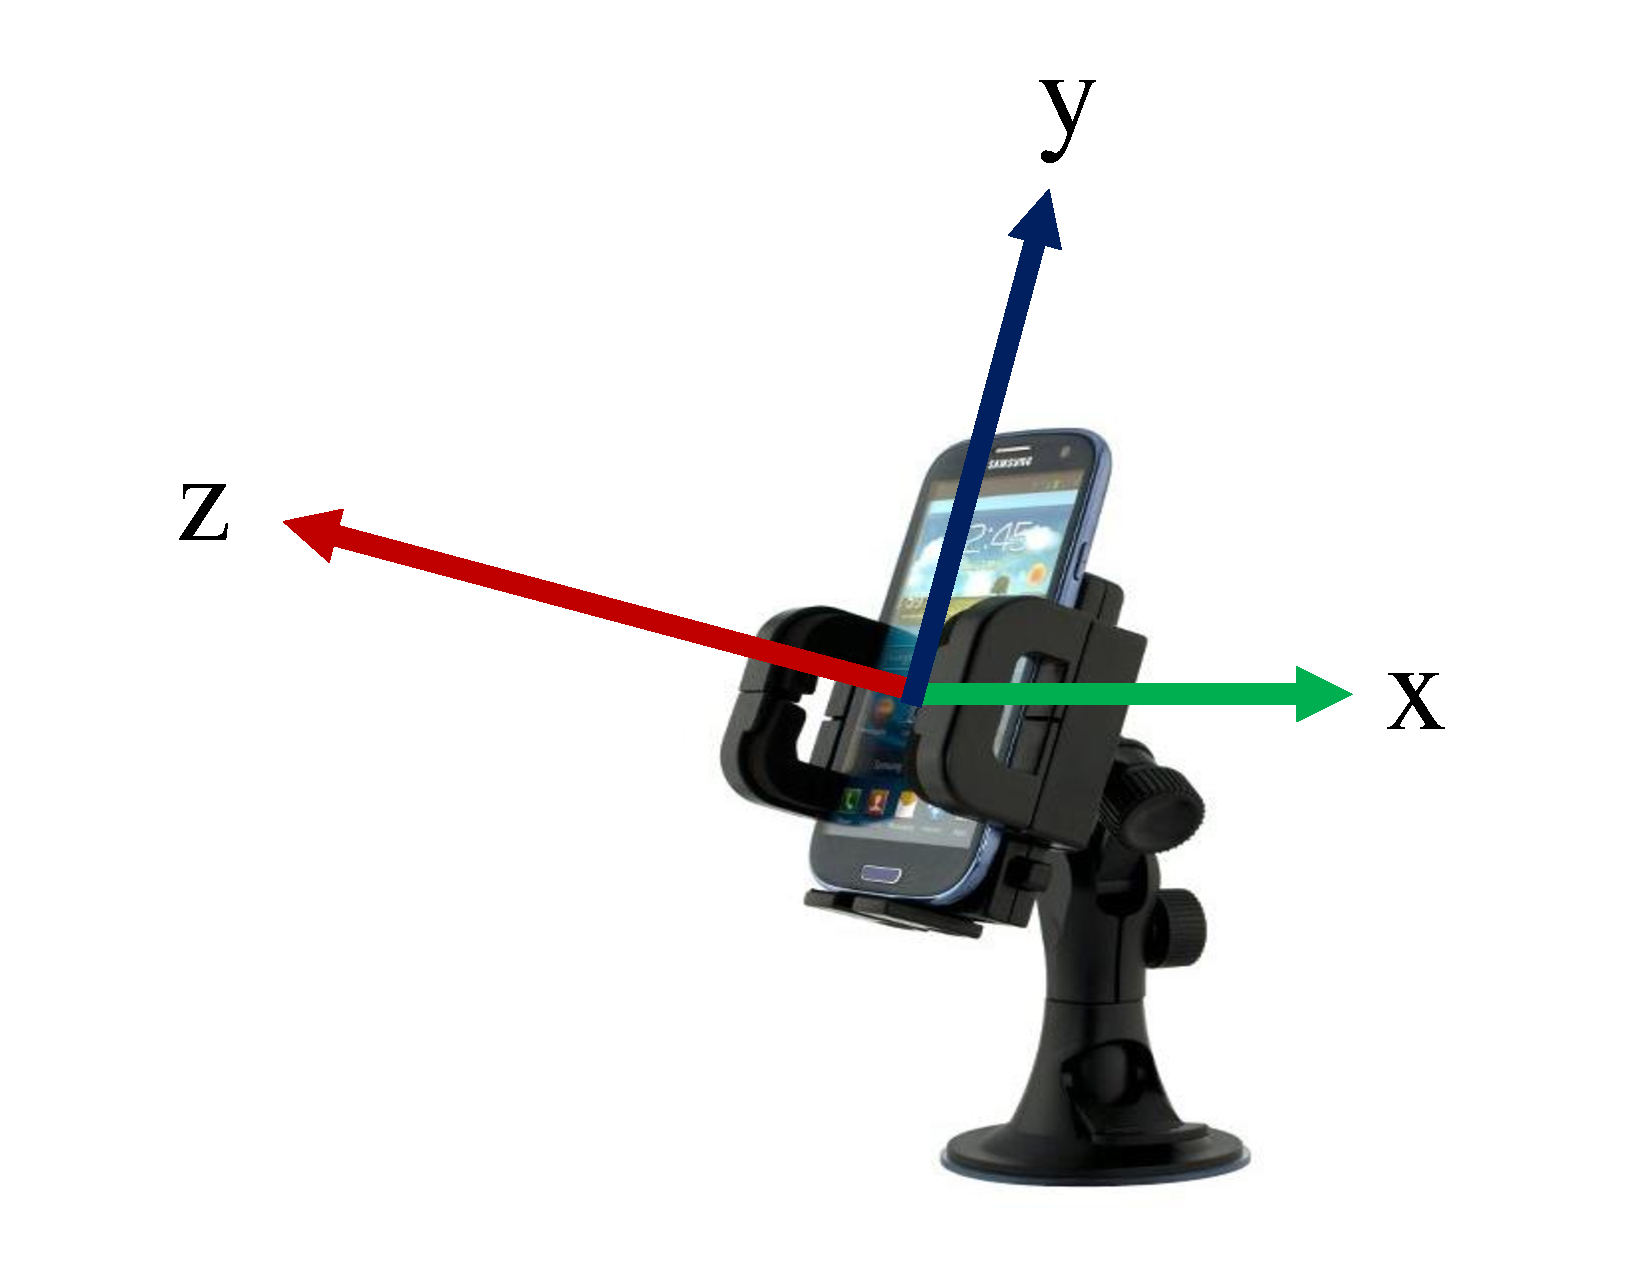
\includegraphics[width=2.8in,angle=0]{Figs/DriveSense/phone3d.pdf}
\vspace{0.0cm}
\hspace{-1.0cm}
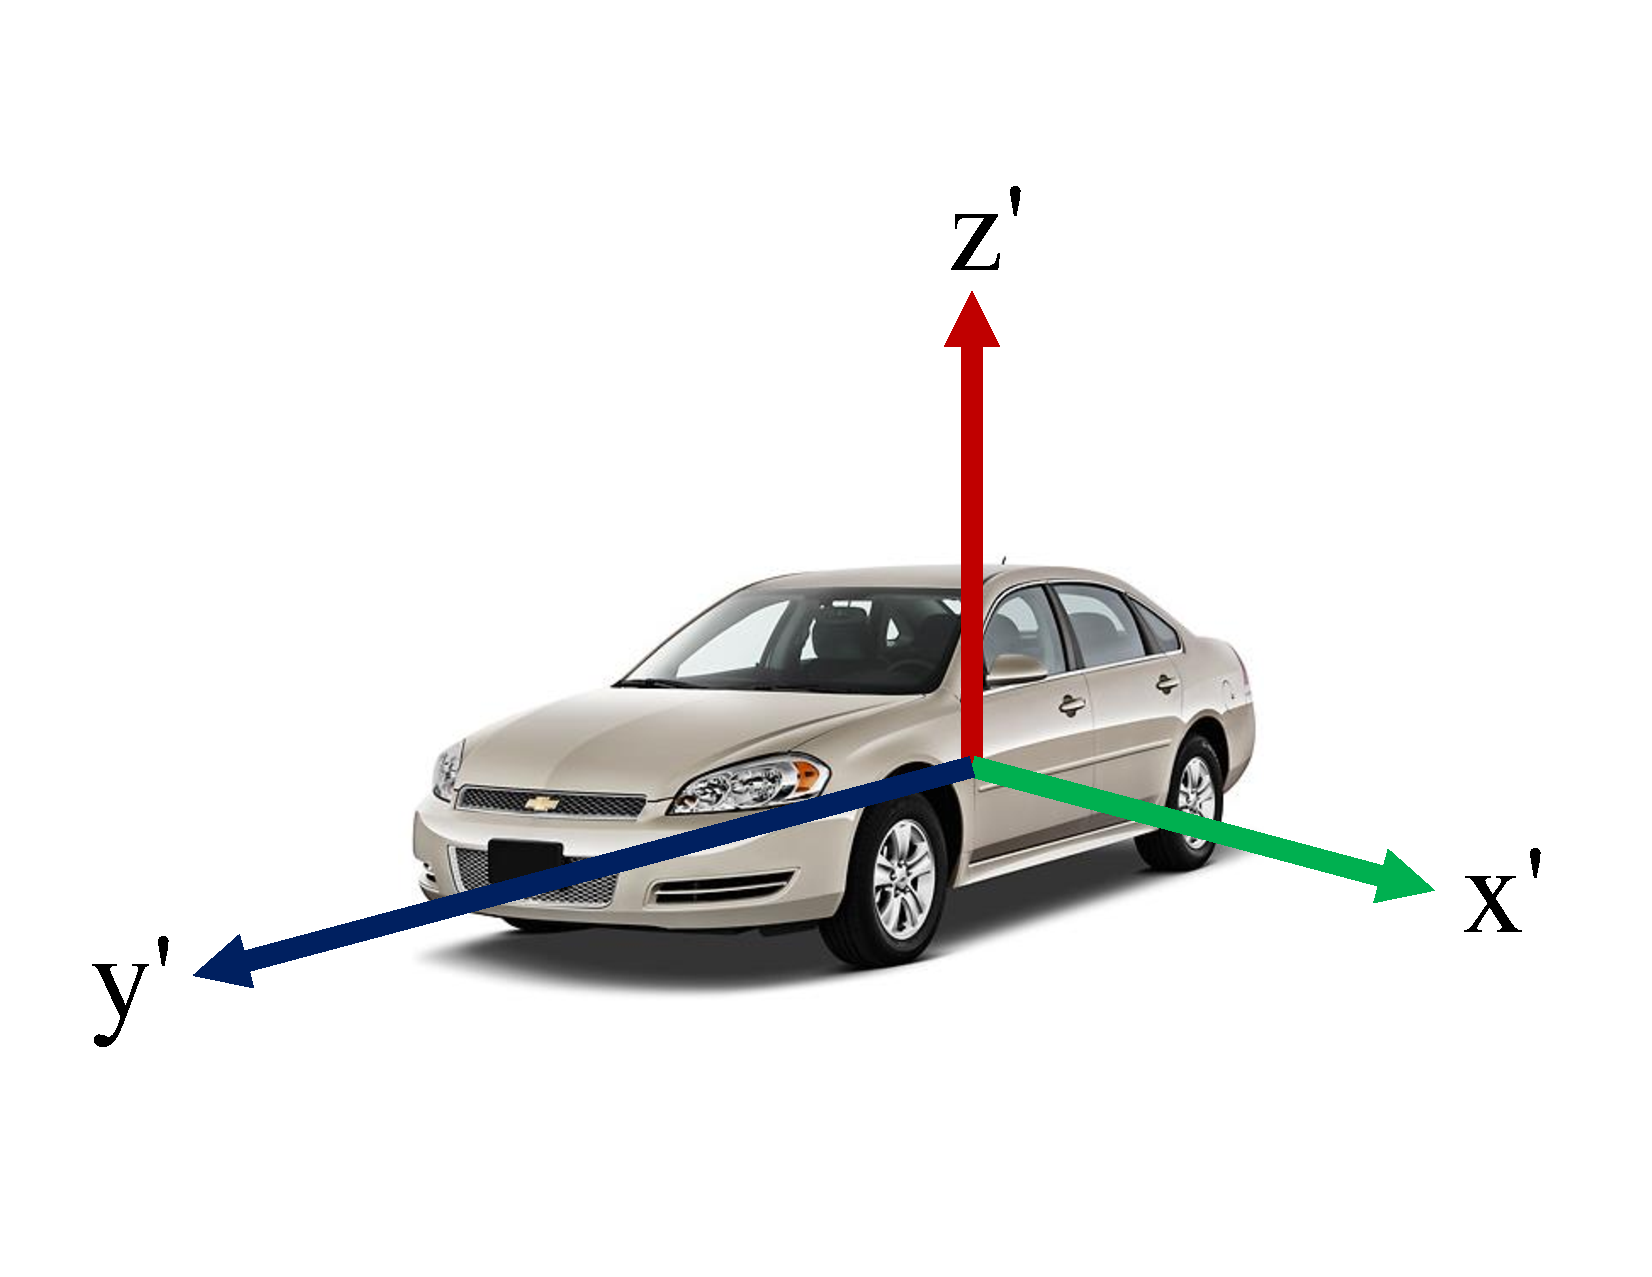
\includegraphics[width=2.8in,angle=0]{Figs/DriveSense/car3d.pdf}
\vspace{-0.2cm}
\caption{Coordinate system difference between a smartphone $[x, y, z]$ and a car $[x', y', z']$.}
\vspace{0.2cm}
\label{coordinates}
\end{figure}


\subsubsection{Slope-Aware Alignment and Linear Acceleration Estimation}


As illustrated in Fig. \ref{coordinates}, we use 
$[x, y, z]$ to represent the three dimensions of a smartphone
and use $[x', y', z']$ to represent the three dimensions
of a car. 
Coordinate alignment is the process that trains the rotation
matrix $R = [\hat{i}, \hat{j}, \hat{k}]$, 
where $\hat{i}$, $\hat{j}$ and $\hat{k}$ are three unit coordinate vectors,
so that $[x', y', z'] = [x, y, z] \times [\hat{i}, \hat{j}, \hat{k}]$.




\textbf{Step 1: Stop Points Extraction}. 

Identifying stop points are useful to conduct an initial alignment. 
We use a sliding window to track the deviation of the
accelerometer readings for this purpose.
The deviation is expected to be small when the car is stopped, 
i.e., in front of stop sign of red traffic light. 
But different cars have different vibrations, 
which affect the readings of the accelerometer. 
To identify a threshold for the deviation, 
we extract the stop points according to the speed information
collected from the OBD port.
We record the start time $s_t$ and end time $e_t$ that 
any speed reading in between is zero. 
To eliminate possible asynchronization and drifted value
after passing low-pass filter, 
we remove the points of the first 500ms and the last 500ms,
i.e., the data points within $[s_t + 500, e_t - 500]$. 
This process helps us to set the threshold to detect
stops. 
We only use OBD as a training input, 
our method can be used on any smartphone and vehicle settings
without OBD inputs. 
 

\textbf{Step 2: Horizontal Alignment}. 


Road slope affects the accuracy of coordinate alignment
in each step. 
During horizontal alignment, a slope-aware alignment method can
be much more effective than a slope-unaware approach. 
As illustrated in Fig. \ref{direction}, 
slope-unaware solutions assume all the data points 
pass the origin point and try to fit all the data
points for a single fit curve, 
while slope-aware solution treats each road segment
as different inputs (deviating from the origin point
due to slopes) and combine to improve the accuracy. 

To train the rotation matrix, we need to select the segments that the car is moving 
straight, and estimate the angle between the 
heading direction and the smartphone's horizontal coordinates \cite{wang2013sensing}.
To derive the rotation matrix from discrete sensor data points, 
we need to fit the curve and find the direction unit vector. 
We propose to train the horizontal
unit vector for each segment and combine each training results gradually with different weights.
There are lots of straight driving segments as illustrated in Fig. \ref{direction}, 
but not all of the segments are good for the training purpose. 
Each segment is selected based on the number of data points that
indicate the car is moving.
The intuition is that more data points could be more statistical significant. 
In Fig. \ref{direction}, we separate four segments and train the 
horizontal unit vector separately.
Clearly, this approach gives better view results that the four slopes of the 
fitting curves are $-0.98$, $-0.87$, $-0.93$ and $-0.95$, respectively. 
The weighted average is $-0.94$. 
After obtain the angle $a$, the horizontal 
rotation matrix can be calculated as follows. 

\[
R_h
	=
\begin{bmatrix}
   cos(\alpha) & -sin(\alpha) & 0 \\
   sin(\alpha) & cos(\alpha) & 0 \\
   0 & 0 & 1
\end{bmatrix}
\]



\begin{figure}[ht] 
\center
\hspace{-0.4cm}
  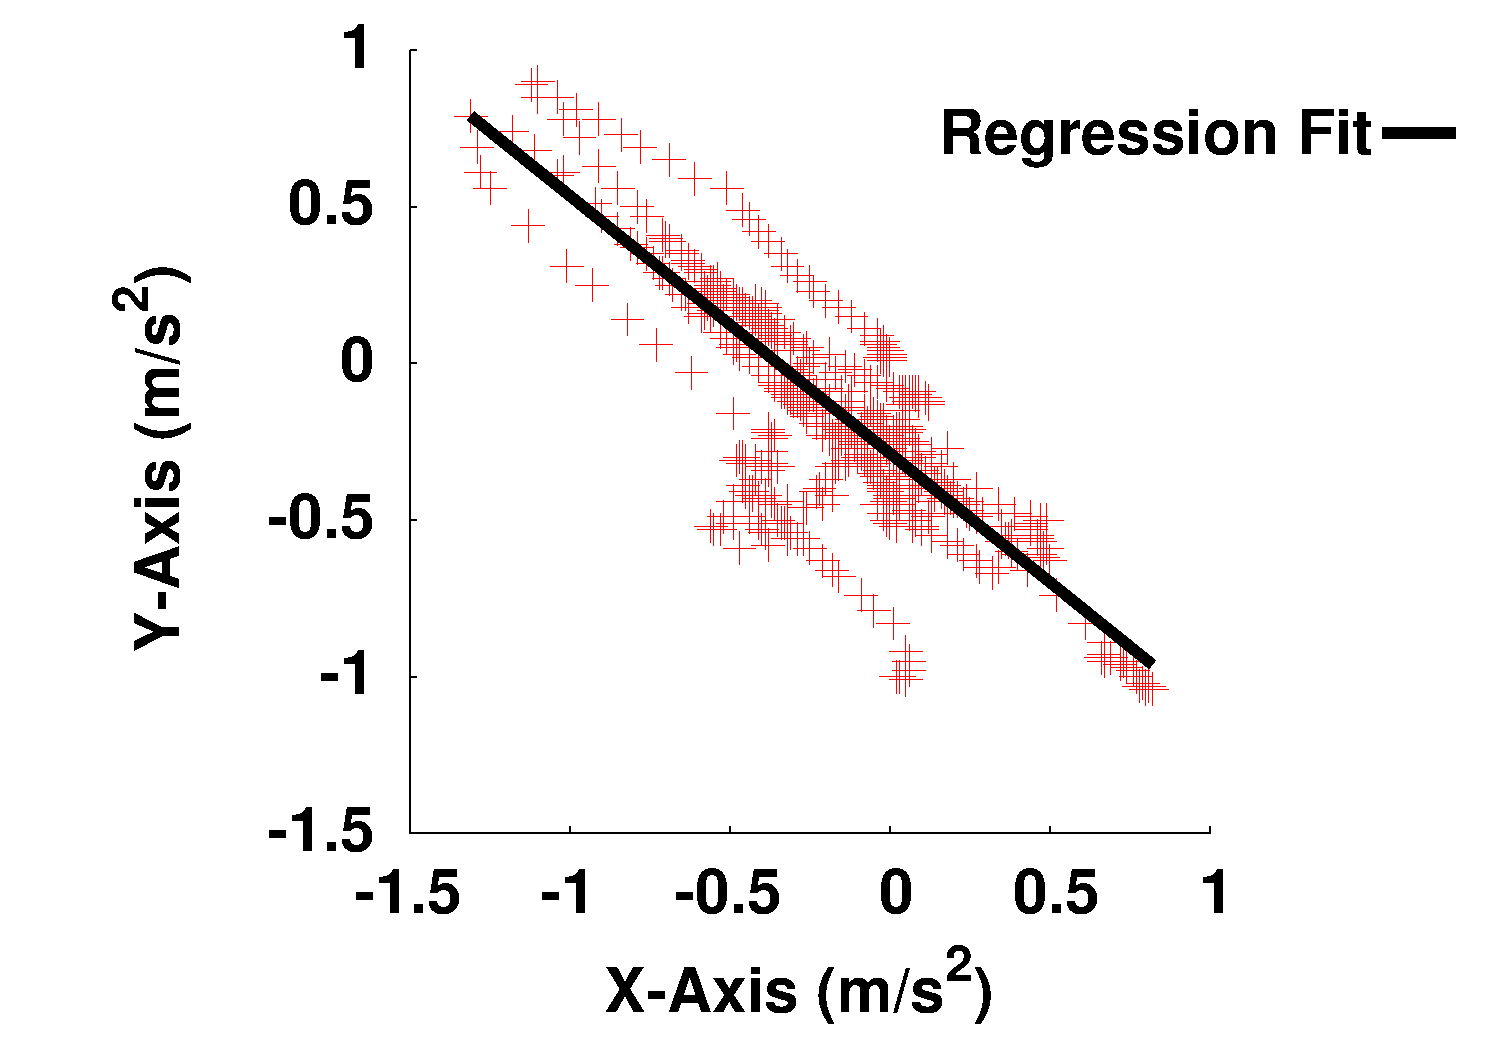
\includegraphics[width=2.6in,angle=0]{Figs/DriveSense/slopeaware/stateoftheart.pdf}
\hspace{-0.0cm}
  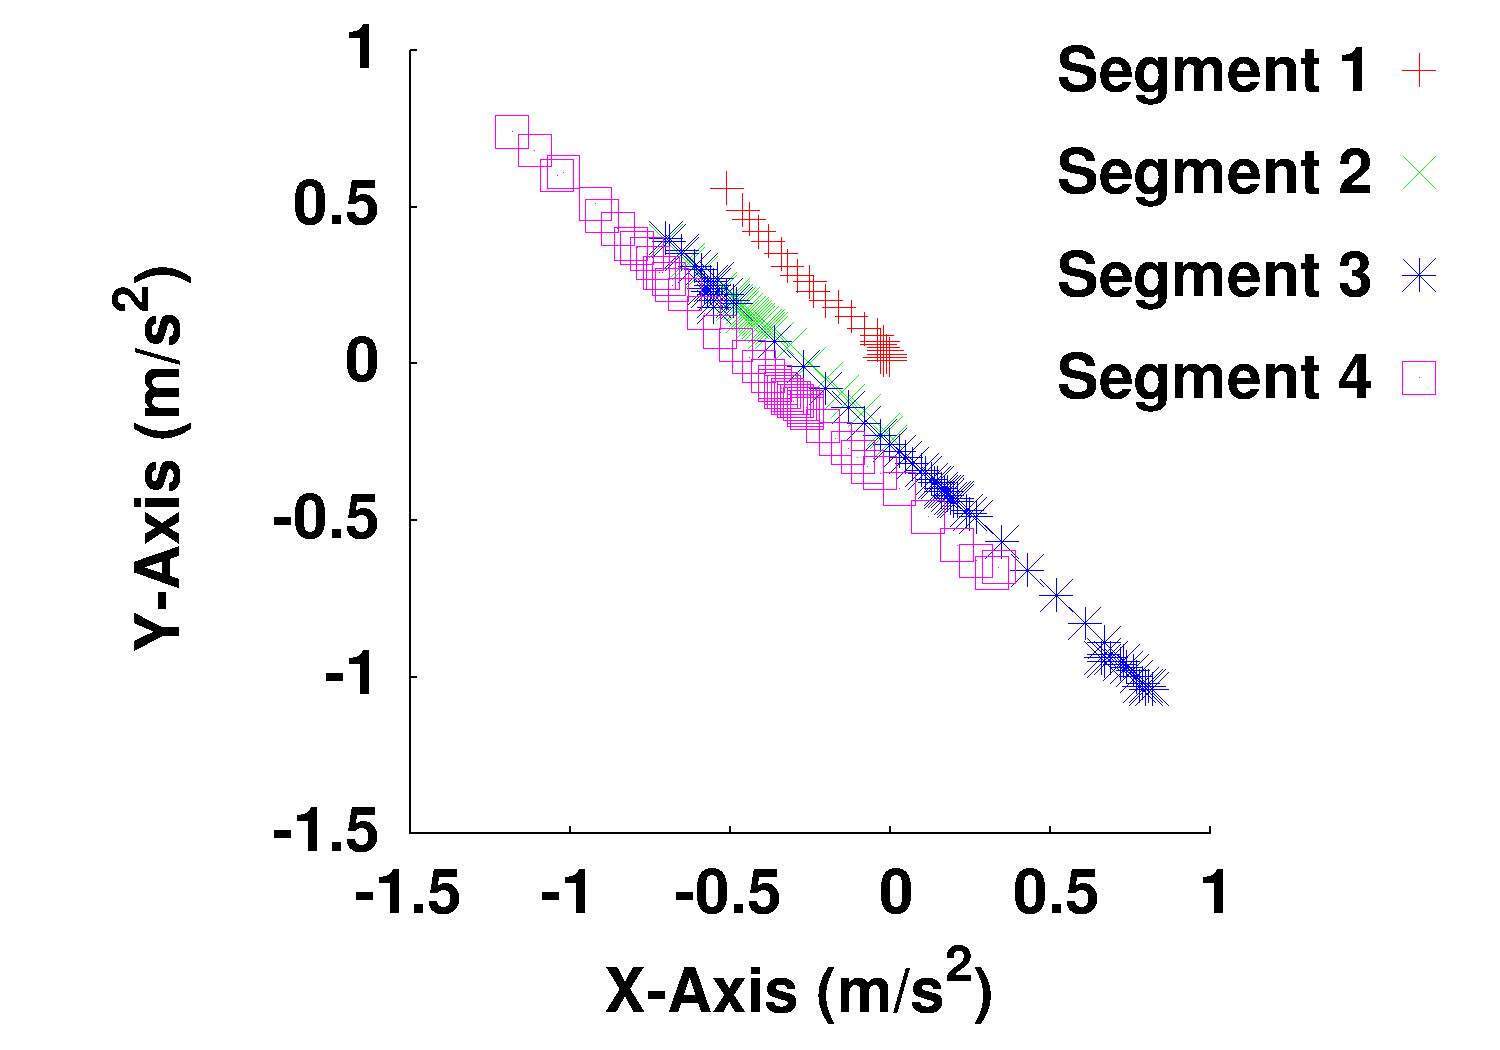
\includegraphics[width=2.6in,angle=0]{Figs/DriveSense/slopeaware/direction.pdf}
\hspace{-0.0cm}
   \caption{Training horizontal rotation matrix by using traditional
approach (above) and slope-aware multi-segment method (below).}
\label{direction}
\vspace{0.4cm}
\end{figure}





\begin{figure}[ht]
\begin{center}
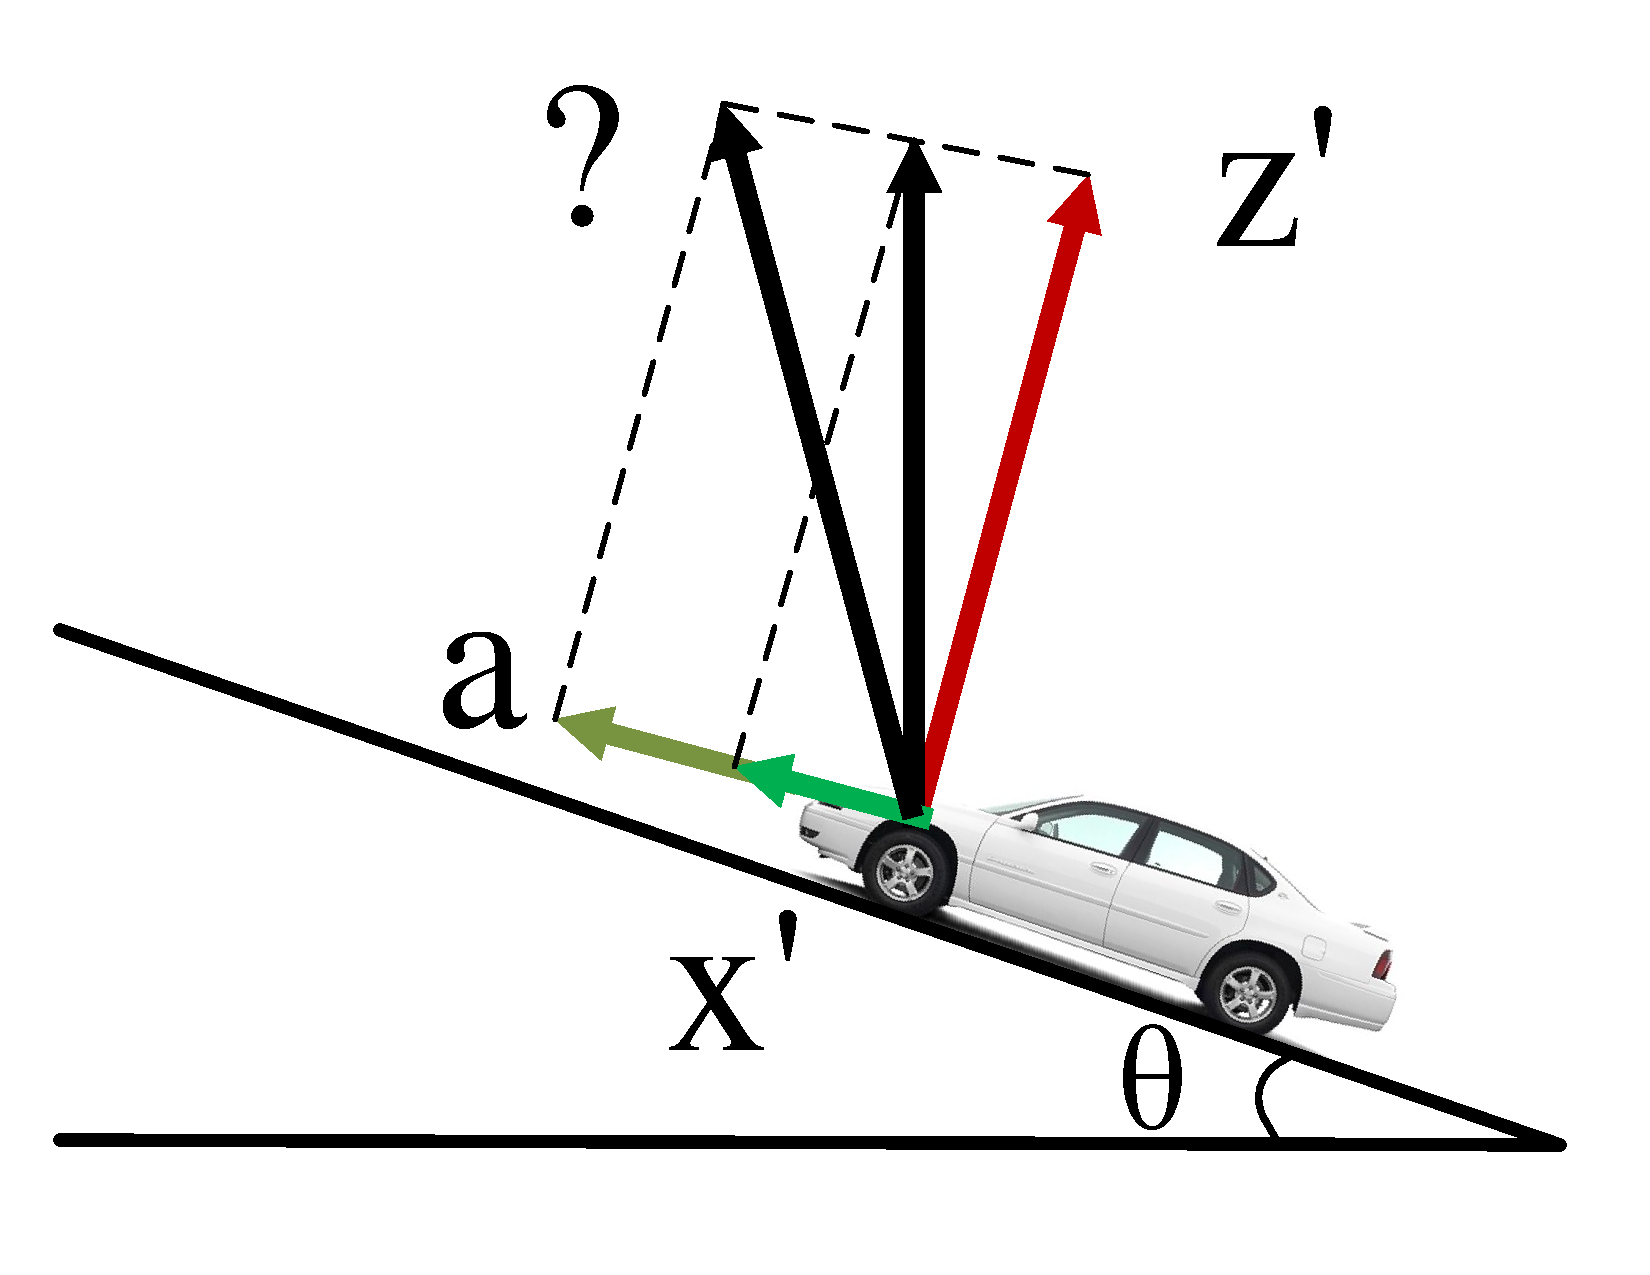
\includegraphics[width=3.0in, angle=0]{Figs/DriveSense/uncertain_vertical.pdf}
\vspace{0.0cm}
	\caption{
Since the actual acceleration of the car 
and the component of gravitational force (along the slope) are unknown, 
the direction of force is uncertain when conducting vertical alignment.
}
\label{training}
\vspace{0.4cm}
\end{center}
\end{figure}




\textbf{Step 3: Slope-Aware Alignment}. 

Estimating road slope at alignment time is challenging. 
In horizontal alignment, we can fit a curve as the moving
direction of the car (or the direction of force) is fixed and not much interfered 
by gravity. 
In vertical alignment, however, the direction of force is changing. 
As illustrated in Fig. \ref{training}, the direction of force changes
as the change of the acceleration of the car. 
There are two parameters are unknown, the slope gradient 
and the vehicle acceleration. 
The vehicle acceleration varies at each data point, 
which varies the direction of force and makes it is very
challenging to estimate the parameters.
We use one heuristic searching algorithm to search for best alignment angle. 
The algorithm relies on the property that the $z'-axis$ of 
the car should be constant over the same slope. 
Firstly, we assume the horizontal alignment is complete and
we convert a 3D alignment problem into a 2D alignment problem. 
The two dimensions are $y-axis$ and $z-axis$, 
as illustrated in Fig. \ref{training}.
By iterating over all the possible angles, 
we calculate deviation of the $z'-axis$ and locate the one with the least deviation. 
The pseudo code of the search algorithm is illustrated in 
Form \ref{search}.




\textbf{Step 4: Linear Acceleration Estimation}.



\begin{figure*}[t]
\begin{center}
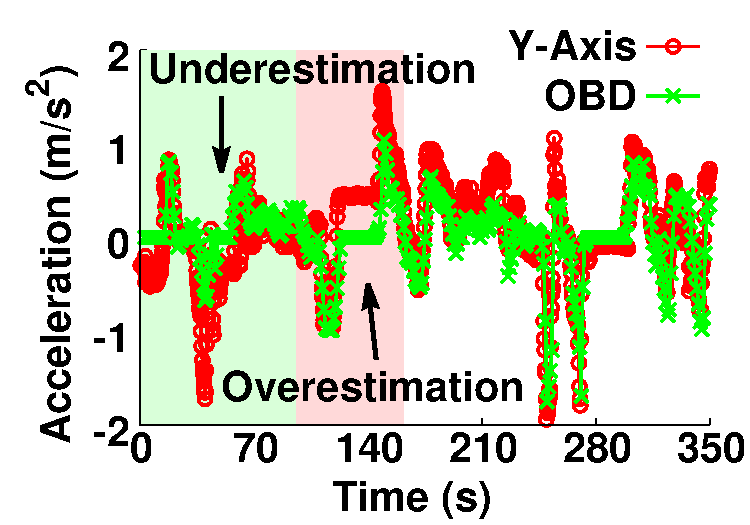
\includegraphics[width=2.0in,angle=0]{Figs/DriveSense/slopeaware/accspeed.pdf}
\hspace{-0.0cm}
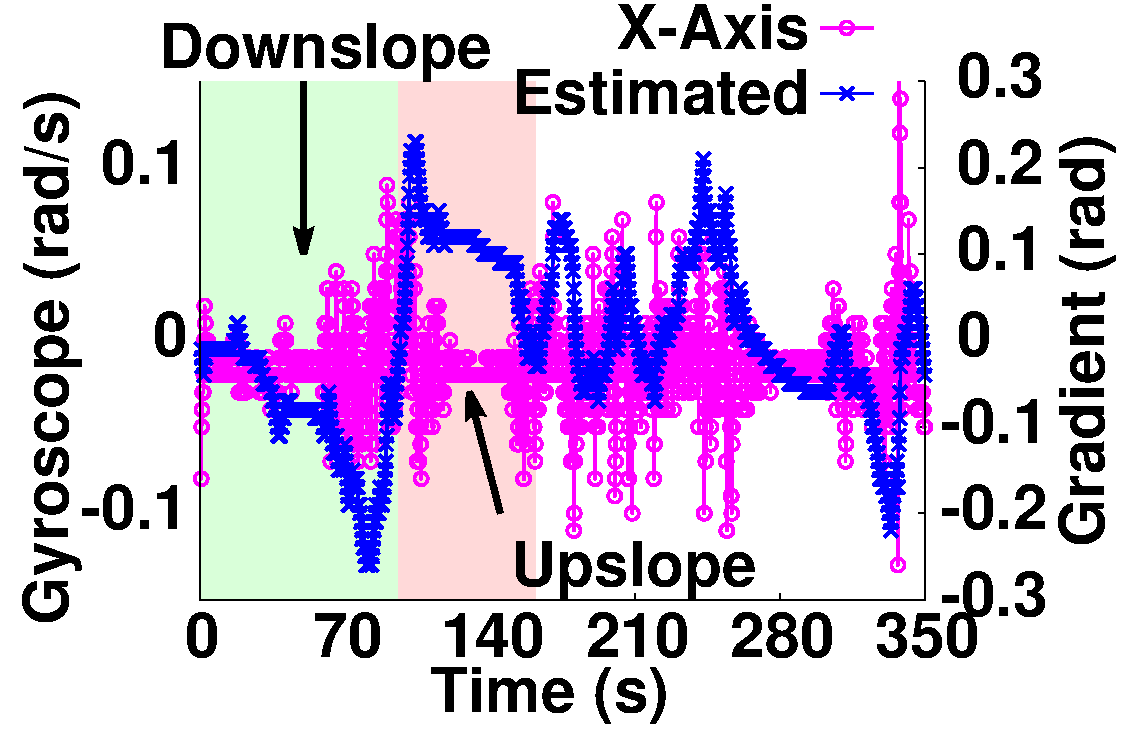
\includegraphics[width=2.0in,angle=0]{Figs/DriveSense/slopeaware/gyrocompare.pdf}
\hspace{-0.0cm}
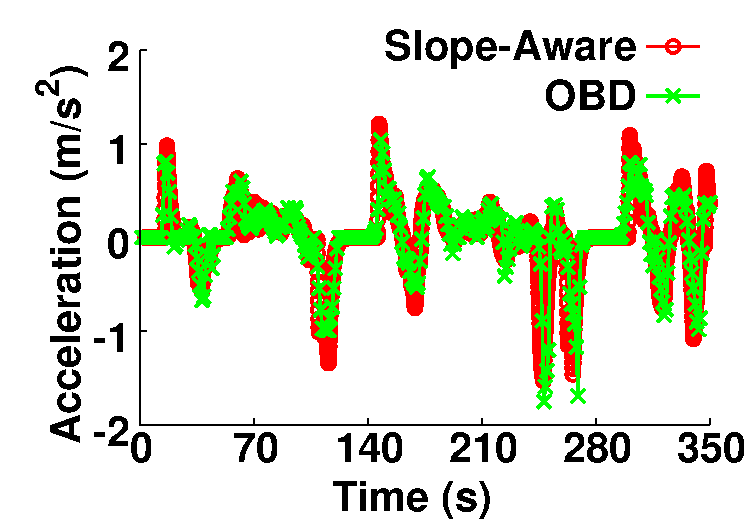
\includegraphics[width=2.0in,angle=0]{Figs/DriveSense/slopeaware/acccompare.pdf}
\hspace{-0.0cm}
\vspace{-0.2cm}
\caption{Slope-Aware coordinate alignment and linear acceleration estimation. 
The Figs/DriveSense are about acceleration over/under estimation caused by slopes (left), 
using gyroscope to estimate road slopes (middle), 
comparing estimated linear acceleration with groundtruth acceleration (right).}
\vspace{-0.2cm}
\label{linear_acceleration}
\end{center}
\end{figure*}


After coordinate alignment is complete, 
we can track the acceleration of a car by using the accelerometer's y-axis. 
We illustrate the acceleration values from aligned accelerometer 
in an example trip illustrated in Fig. \ref{linear_acceleration}. 
As the figure shows, comparing with the accelerations by OBD,   
the accelerations by the accelerometer of the first $90s$ 
are underestimated and the following $60s$ are overestimated.
This is because the car is moving mainly downslope and then mainly upslope. 
The deviated estimations may cause false positives/negatives on 
capturing driving behaviors such as brakes and accelerations.

We apply the same rotation matrix to the gyroscope data and 
illustrate the gyroscope x-axis data in Fig. \ref{linear_acceleration}.
After removing the constant drifts, 
it shows clear trends that the car is moving downslope and then
upslope.
Given the similar trends illustrated in two plots, 
we can estimate the slope gradient and deduct the gravitational force
components. 
We use similar calibration techniques proposed in \cite{zhou2014use}. 
We identify the road segments and stop points where accelerometer
can provide more accurate slope gradients to calibrate gyroscope.  


